\documentclass[10pt,english]{article}
\usepackage[T1]{fontenc}
\usepackage[latin9]{inputenc}
\usepackage[a4paper]{geometry}
\geometry{verbose}
\pagestyle{plain}
\usepackage{babel}
\usepackage{graphicx}

\usepackage{amsmath}
\usepackage{setspace}
\onehalfspacing
\usepackage[unicode=true, pdfusetitle,
 bookmarks=true,bookmarksnumbered=false,bookmarksopen=false,
 breaklinks=false,pdfborder={0 0 1},backref=false,colorlinks=false]
 {hyperref}

\usepackage{mathpazo}
\usepackage{siunitx}
\usepackage{microtype}
\usepackage{nicefrac}

\begin{document}

%\author{Gen Zhang}
\title{Notes on spinal chord structure and development}

\maketitle

\section{Tissue organisation}

During development, the spinal chord grows from the anterior towards the
posterior. At the same time, somites develop parallel to the neural tube.
Observations indicate that labelled cells in the spinal chord and somites
remain parallel as development proceeds. It seems reasonable to believe that 
the posterior end lays down tissue as it moves. Nevertheless, there is
considerable growth of the somites, and so there should still be considerable
growth even away from the posterior end. The protocol is thus to take transverse slices at the same somite number and track as development proceeds.

The spinal chord itself forms a pseudo-stratified tissue, in which cells migrate
to the apical surface when they undergo mitosis. We may at least divide cells
into two types: progenitors and mature neurons. These may be defined in three
ways:

\begin{enumerate}
\item lineage --- progenitors will divide again, mature neurons do not;
\item morphology --- progenitors are less round, more elongated;
\item labelling --- progenitors are sox2 (?) positive; mature neurons are p27
	positive.
\end{enumerate}

We shall ignore morphology from now on because it is too qualitative, and do not
provide a sufficiently precise definition. It is important to note that these do 
not necessarily correspond to the same definitions; further, this is not an
academic question because our experimental data will use both, and we need to be
clear about which one is being used to explain what we see.

From here on, the word \emph{progenitor} will refer to cells capable of division,
and those defined by labelling will be referred to as \emph{sox2 +ve} or 
\emph{sox2 -ve} (p27 is not as tight a marker (?)). 

It is observed (?) that division only occurs for cells displaying sox2; or
rather that sox2 -ve cells are definitely \emph{not} capable of division. We can 
then postulate the existence of cells committed to differentiation but still
sox2 +ve, i.e. post-mitotic cell. Thus overall, we are talking about the 
division process:

\begin{figure}[h]
	\begin{center}
		\includegraphics[width=4in]{division-process-A.pdf}
	\end{center}
\end{figure}

Note that the parameters marked above refer to averages, and also may depend
on time, fate, siblings, etc.

\paragraph{Caveat 1}

Everything depends on cell fate being determined at division. This specifically
rules out a process where a progenitor can chose to simply differentiate without
division, e.g. a progenitor will no longer divide if it has not in the first 50
hours of its life, and will then just differentiate. I'm aware that such a
scenario is popular in the neurogenisis field, and maybe I need to be educated.
In any case, see below, section ``Model B''.

Through the use of other markers (?) it is possible to distinguish four types
of differentiated cells. Further, sox2 +ve cells also display these markers.
These different types of cells exist in spatially separate domains arranged
along the dorso-ventral axis.

\begin{figure}[h]
	\begin{center}
		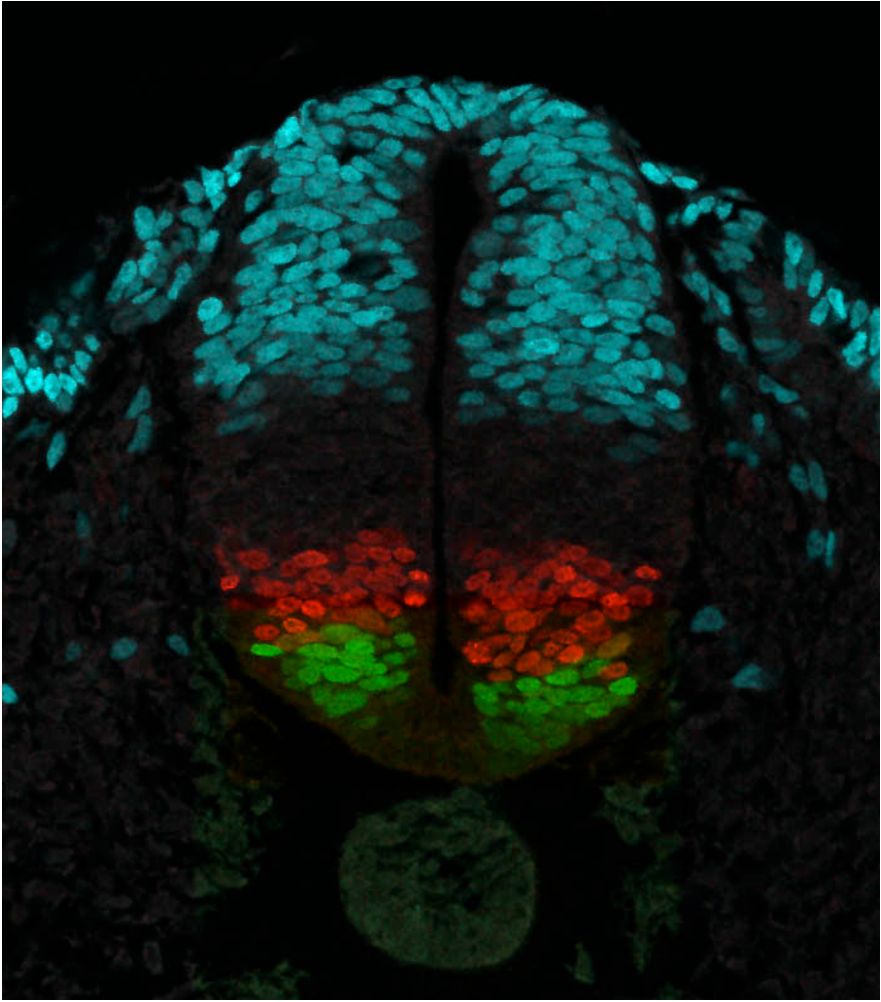
\includegraphics[height=2.5in]{transverse-stained-domains.pdf}
		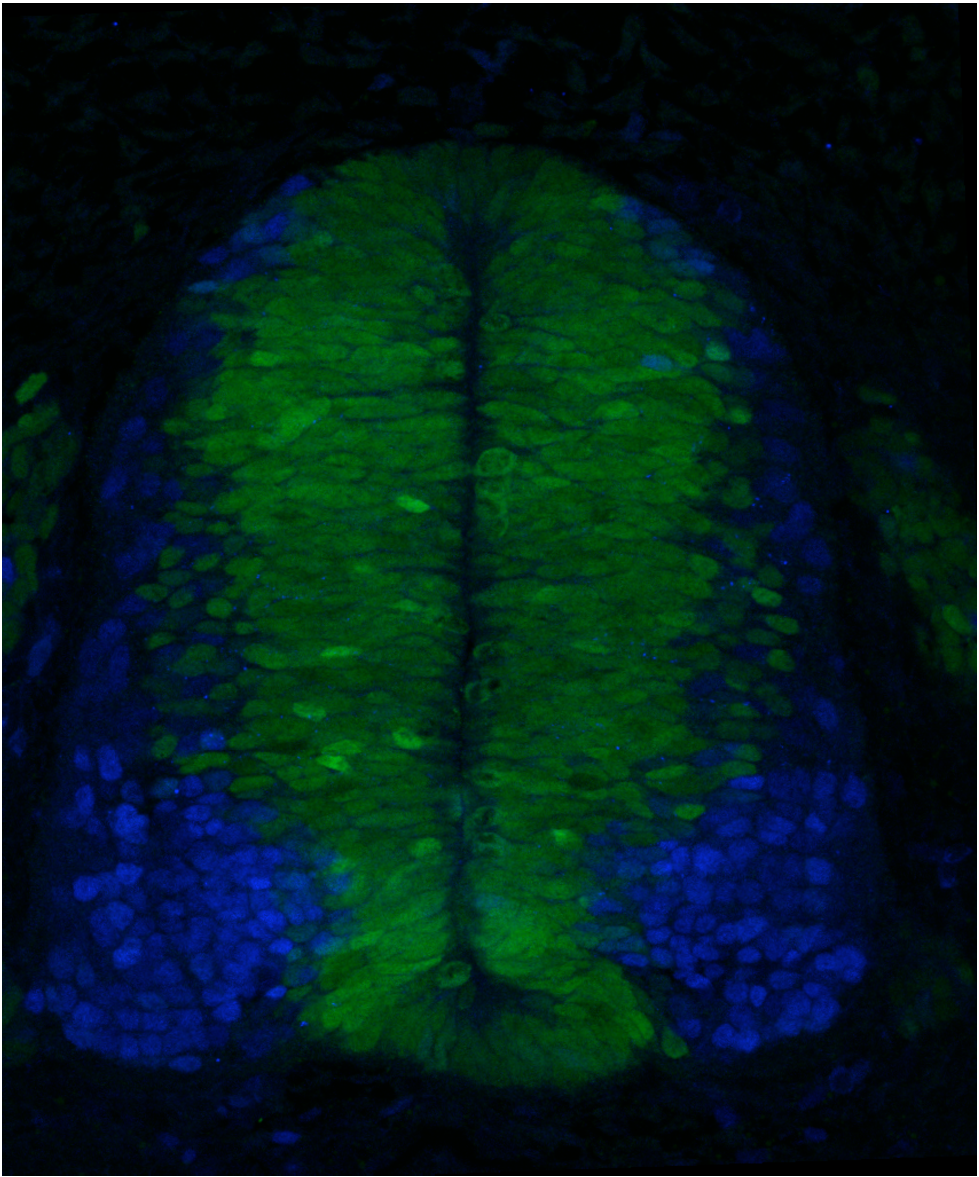
\includegraphics[height=2.5in]{transverse-stained-sox2-p27.pdf}
	\end{center}
\end{figure}

It is thought that these markers are set up as a result of a hedgehog gradient (?)
and may be influential in regulating the growth.

\section{Cell cycle and fate choice is independent of fate}

We can try and spot cells undergoing mitosis with PH3 staining of flat mounts.
This gives us a measure in terms of number of cells undergoing mitosis (in the
sense of being PH3 +ve) per unit area, $m^\textrm{PH3}$. We may also count the
number of sox2 +ve cells per unit area in transverse sections (in the apical-
basal/dorvo-ventral plane), $p^\textrm{sox2}$; the sections are of thickness $s$. 
We must then have the identity
$$ \frac{\tau^\textrm{ph3}_\textrm{mit.}}{\tau_\textrm{cycle}} = 
	\frac{s[DV][AB]}{\rho p^\textrm{sox2}} \frac{m^\textrm{PH3}}{[AB]} $$
where $[DV]$ is the physical dimension of the domain in the dorso-ventral axis,
$[AB]$ is the dimension in the apico-basal axis, and $\rho$ is the proportion of 
sox2 +ve cells which are progenitors.

\paragraph{Caveat 2}

There is a rather subtle issue of whether the volume density of sox2 +ve cells
is given by $p^\textrm{sox2}/s[DV][AB]$. Clearly, for a large $s$ (section thickness
much larger than cell dimension), this is correct --- doubling the thickness
will double the number of cells per section. However, for infinitesimal slices, 
doubling the thickness will give exactly the same number of cells. Annoyingly,
the cross over will occur when the section thickness is about the same as cell
dimension. To resolve this I need to understand in greater detail what the
protocol is for counting cells in each section.

Everything on the right-hand side, apart from $\rho$, can be measured. We can
then calculate and plot the quantity $\rho \tau^\textrm{ph3}_\textrm{mit.}/\tau_\textrm{cycle}$
for each domain as a function of time:

\begin{figure}[h]
	\begin{center}
		\includegraphics[width=3in]{rhoph3taus.eps}
	\end{center}
\end{figure}

Furthermore, it is also possible to make another measure of mitosis by directly
spotting cells undergoing mitosis from transverse slices; this gives a 
proportion $m$, and is equal to $\rho \tau_\textrm{mit.}/\tau_\textrm{cycle}$.
Note that $\tau_\textrm{mit.} \neq \tau^\textrm{ph3}_\textrm{mit.}$. Plotting
this again for the different domains as a function of time:

\begin{figure}[h]
	\begin{center}
		\includegraphics[width=3in]{rhotaus.eps}
	\end{center}
\end{figure}

The main result is that all domains behave the same. There is also a drop of a 
factor of a few over the time course. The quantitative difference between the
two measurements can be understood to be a result of different definitions of
mitosis.

Given that the sox2 +ve cells display the differentiation type markers, it
might be thought that the division process could be dependent on the type of
marker. However, the results from direct mitotic index measurements suggest that actually cell division is independent of which domain the progenitors reside in.

The drop in the combined quantity, $\rho \tau_\textrm{mit.} / \tau_\textrm{cycle}$,
is significant. We can assume that mitosis duration is constant. We thus need
to reconcile the difference (2--10 fold) in changes to $\rho$ and/or
$\tau_\textrm{cycle}$. \emph{Is this reasonable?}

There is now an intriguing possibility. We have strong(-ish) evidence that the
differentiation marker does not seem to effect the division rate/process in
general. If we accept that a differentiated cell (p27 +ve) has its fate 
determined already by the differentiate type marker it expresses, we can still ask
if the progenitors are destined to produce only cells of one type.

We can test this decoupling further by considering the relative growth of each 
domain. If the domains were independent, then the total number of cells, both 
sox2 +ve and -ve, as a proportion of the final total number of cells, should 
grow in the same way independently of domain:

\begin{figure}[h]
	\begin{center}
		\includegraphics[width=3in]{growth-fraction.eps}
	\end{center}
\end{figure}

\paragraph{Comment}

Here I've actually cheated and and adjusted the scale for each line by hand.
Things look even worse if I just naively scale by the final count. The important
thing is that \emph{sometimes the count goes down}. Admittedly, things are
always within error bars (though intermediate at around 55 hours seems to 
\emph{really} decrease). (Why are the errorbars so large? Most of the error is
coming from neuron counts. Is that trying to tell us something?)

Currently, it looks like the independence hypothesis is not correct, implying
that progenitors can switch their differentiation type marker. (Are we sure
that p27+ cells are not able to change too?) An excellent experimental signature
would be to see clones of progenitors displaying heterogenous differentiation
type markers.

\section{Accuracy}

Currently, the error bars associated with some of the measurements are rather
large. From the battery of measurements available, we can construct a consistency
check in the form of ``progenitor cell depth''. This quantity should simply be
roughly the dimension of a sox2 +ve cell measured in the anterior-posterior axis.
We expect, from observations, that this should be a tightly distributed quantity,
independent of both space and time variations. Since this quantity depends
on both number counts and size measurements, it is a good indicator of accuracy:

\begin{figure}[h]
	\begin{center}
		\includegraphics[width=2.8in]{cell-depth.eps}
		\hfill
		\includegraphics[width=2.8in]{cell-depth-hist.eps}
	\end{center}
\end{figure}

For example, we see that there is a correlated spike at $\sim 58$ hours, and an
outlier in p3 at $70$ hours. Unfortunately, I have not worked out what exactly
caused them.

\section{Model B}

There is an interesting limit of the division process, which considerably
simplifies things. When transit time of sox2 +ve post-mitotic cells is very
short, we can simply ignore their existence. This is equivalent to setting
$\rho = 1$. Further, if the decision to differentiate is actually taken after
division, then we have the property that $r_2 = \left(1 - \sqrt{r_1} \right)^2$. 
In this case, the process is equivalent to:

\begin{align*}
P &\overset{\lambda}{\longrightarrow} P+P \\
P &\overset{\gamma}{\longrightarrow} N
\end{align*}

However, in view of measurements of mitotic index, it would mean that all the
change in $\rho \tau_\textrm{mit.} / \tau_\textrm{cycle}$ needs to be taken up
by change in $\tau_\textrm{cycle}$. Is a five-fold change reasonable?

\end{document}
